%
% $File: report.tex
% $Date: Mon Jan 06 00:40:42 2014 +0800
%

\documentclass{article}
\usepackage{fontspec}
\usepackage{zhspacing,url,amsmath,amssymb,verbatim}
\usepackage{pdfpages}
\zhspacing
\usepackage{listings}
\usepackage[hyperfootnotes=false,colorlinks,linkcolor=blue,anchorcolor=blue,citecolor=blue]{hyperref}
\usepackage[backend=biber]{biblatex}
\usepackage{graphicx}
\usepackage{minted}
\usepackage{subfigure}
\usepackage{indentfirst}
\usepackage{cases}
\usepackage{float}			% don't automatically change location of figure [H]
\usepackage{chngpage}		% use \changetext to change page size
\usepackage{environ}
\usepackage{array}
\usepackage[top=1in, bottom=1in, left=1.25in, right=1.25in]{geometry}
\usepackage{caption}\captionsetup{hypcap=true}  % ref to jump to object instead of caption
\newfontfamily\zhfont[BoldFont=SimHei,ItalicFont=KaiTi_GB2312]{SimSun}
\lstset{keywordstyle=\color{blue!70}, commentstyle=\color{red!50!green!50!blue!50},frame=shadowbox,rulesepcolor=\color{red!20!green!20!blue!20},
basicstyle=\footnotesize\ttfamily}

\setlength{\parindent}{2em}

% $File: mint-defs.tex
% $Date: Sun Nov 17 23:37:24 2013 +0800
% $Author: Xinyu Zhou <zxytim@gmail.com>

\newcommand{\inputmintedConfigured}[3][]{\inputminted[fontsize=\footnotesize,
	label=#3,linenos,frame=lines,framesep=0.8em,tabsize=4,#1]{#2}{#3}}

\newcommand{\txtsrc}[2][]{\inputmintedConfigured[#1]{text}{#2}}
\newcommand{\txtsrcpart}[4][]{\txtsrc[firstline=#3,firstnumber=#3,lastline=#4,#1]{#2}}

\newcommand{\cppsrc}[2][]{\inputmintedConfigured[#1]{cpp}{#2}}
\newcommand{\cppsrcpart}[4][]{\cppsrc[firstline=#3,firstnumber=#3,lastline=#4,#1]{#2}}

\newcommand{\javasrc}[2][]{\inputmintedConfigured[#1]{java}{#2}}
\newcommand{\javasrcpart}[4][]{\javasrc[firstline=#3,firstnumber=#3,lastline=#4,#1]{#2}}

\newcommand{\matlabsrc}[2][]{\inputmintedConfigured[#1]{matlab}{#2}}
\newcommand{\matlabsrcpart}[4][]{\matlabsrc[firstline=#3,firstnumber=#3,lastline=#4,#1]{#2}}

\newcommand{\pysrc}[2][]{\inputmintedConfigured[#1]{matlab}{#2}}
\newcommand{\pysrcpart}[4][]{\matlabsrc[firstline=#3,firstnumber=#3,lastline=#4,#1]{#2}}

%\usepackage[T1]{fontenc}
\usepackage{lmodern}
\usepackage{amssymb,amsmath}
\usepackage{ifxetex,ifluatex}
\usepackage{fixltx2e} % provides \textsubscript
% use upquote if available, for straight quotes in verbatim environments
\IfFileExists{upquote.sty}{\usepackage{upquote}}{}
\ifnum 0\ifxetex 1\fi\ifluatex 1\fi=0 % if pdftex
  \usepackage[utf8]{inputenc}
\else % if luatex or xelatex
  \usepackage{fontspec}
  % commented by Xinyu Zhou
  \ifxetex
    \usepackage{xltxtra,xunicode}
  \fi
  \defaultfontfeatures{Mapping=tex-text,Scale=MatchLowercase}
  \newcommand{\euro}{€}
\fi
% use microtype if available
\IfFileExists{microtype.sty}{\usepackage{microtype}}{}
\usepackage{color}
\usepackage{fancyvrb}
\newcommand{\VerbBar}{|}
\DefineShortVerb[commandchars=\\\{\}]{\|}
\DefineVerbatimEnvironment{Highlighting}{Verbatim}{commandchars=\\\{\}}
% Add ',fontsize=\small' for more characters per line
\newenvironment{Shaded}{}{}
\newcommand{\KeywordTok}[1]{\textcolor[rgb]{0.00,0.44,0.13}{\textbf{{#1}}}}
\newcommand{\DataTypeTok}[1]{\textcolor[rgb]{0.56,0.13,0.00}{{#1}}}
\newcommand{\DecValTok}[1]{\textcolor[rgb]{0.25,0.63,0.44}{{#1}}}
\newcommand{\BaseNTok}[1]{\textcolor[rgb]{0.25,0.63,0.44}{{#1}}}
\newcommand{\FloatTok}[1]{\textcolor[rgb]{0.25,0.63,0.44}{{#1}}}
\newcommand{\CharTok}[1]{\textcolor[rgb]{0.25,0.44,0.63}{{#1}}}
\newcommand{\StringTok}[1]{\textcolor[rgb]{0.25,0.44,0.63}{{#1}}}
\newcommand{\CommentTok}[1]{\textcolor[rgb]{0.38,0.63,0.69}{\textit{{#1}}}}
\newcommand{\OtherTok}[1]{\textcolor[rgb]{0.00,0.44,0.13}{{#1}}}
\newcommand{\AlertTok}[1]{\textcolor[rgb]{1.00,0.00,0.00}{\textbf{{#1}}}}
\newcommand{\FunctionTok}[1]{\textcolor[rgb]{0.02,0.16,0.49}{{#1}}}
\newcommand{\RegionMarkerTok}[1]{{#1}}
\newcommand{\ErrorTok}[1]{\textcolor[rgb]{1.00,0.00,0.00}{\textbf{{#1}}}}
\newcommand{\NormalTok}[1]{{#1}}
% \ifxetex
%   \usepackage[setpagesize=false, % page size defined by xetex
%               unicode=false, % unicode breaks when used with xetex
%               xetex]{hyperref}
% \else
%   \usepackage[unicode=true]{hyperref}
% \fi
\hypersetup{breaklinks=true,
            bookmarks=true,
            pdfauthor={},
            pdftitle={},
            colorlinks=true,
            urlcolor=blue,
            %linkcolor=magenta,
            pdfborder={0 0 0}}
%\urlstyle{same}  % don't use monospace font for urls
\setlength{\parindent}{0pt}
\setlength{\parskip}{6pt plus 2pt minus 1pt}
\setlength{\emergencystretch}{3em}  % prevent overfull lines
%\setcounter{secnumdepth}{0}



\newcommand{\figref}[1]{\hyperref[fig:#1]{Figure.\ref*{fig:#1}}}
\newcommand{\eqnref}[1]{\hyperref[eqn:#1]{Equation.\ref*{eqn:#1}}}
\newcommand{\tableref}[1]{\hyperref[table:#1]{Table.\ref*{table:#1}}}
\newcommand{\centerize}[1]{\begin{center} #1 \end{center}}
\newcommand{\secref}[1]{\hyperref[sec:#1]{Section.\ref*{sec:#1}}}
\newcommand{\appref}[1]{\hyperref[app:#1]{App.\ref*{app:#1}}}


\usepackage{fancyhdr}
\changetext{}{2.2cm}{-1.1cm}{-1.1cm}{}
\pagestyle{fancy}
\setlength{\headheight}{15.2pt}
\lhead[]{}\rhead[]{}
\fancyhead[C]{\emph{Speaker Recognition}}

% math function
\let\Oldsum\sum
\renewcommand{\sum}{\displaystyle\Oldsum}
\let\Oldprod\prod
\renewcommand{\prod}{\displaystyle\Oldprod}


\newcommand{\cmd}[1]{{\it #1}}
\newcommand{\ccmd}[1]{\centerize{\cmd{#1}}}

\title{Digital Signal Processing: Speaker Recognition \\ Final Report \\ (Complete Version)}
\author{Xinyu Zhou, Yuxin Wu, and Tiezheng Li\\ Tsinghua University}
\date{}

\bibliography{refs.bib}
\begin{document}

\fontsize{11pt}{1.4em}
\setlength{\baselineskip}{1.6em}
\maketitle
\tableofcontents


\defbibheading{bibliography}{\section{References}}
%thick shline
\newlength\savewidth
\newcommand\shline{\noalign{\global\savewidth\arrayrulewidth\global\arrayrulewidth 1pt}
                   \hline
                   \noalign{\global\arrayrulewidth\savewidth}}


\section{Introduction}
A \textbf{Speaker Recognition} tasks can be classified with respect to different criterion:
Text-dependent or Text-independent, Verification (decide whether the person is he claimed to be) or Identification (decide who the person is by its voice).\cite{SRwiki}

Speech is a kind of complicated signal produced as a result of several transformations occurring at different levels: semantic, linguistic and acoustic.
Differences in these transformations may lead to differences in the acoustic properties of the signals.
The recognizability of speaker can be affected not only by the linguistic message
but also the age, health, emotional state and effort level of the speaker.
Background noise and performance of recording device also interfere
the classification process.

Speaker recognition is an important part of Human-Computer Interaction (HCI).
As the trend of employing wearable computer reveals,
Voice User Interface (VUI) has been a vital part of such computer.
As these devices are particularly small, they are more likely to lose and be stolen.
In these scenarios, speaker recognition is not only a good HCI,
but also a combination of seamless interaction with computer and security guard
when the device is lost.
The need of personal identity validation will become more acute in the future.
Speaker verification may be essential in business telecommunications.
Telephone banking and telephone reservation services will develop rapidly
when secure means of authentication were available.

Also,the identity of a speaker is quite often at issue in court cases.
A crime victim may have heard but not seen the perpetrator,
but claim to recognize the perpetrator as someone whose voice was previously familiar;
or there may be recordings of a criminal whose identity is unknown.
Speaker recognition technique may bring a reliable scientific determination.

Furthermore, these techniques can be used in environment which demands high security.
It can be combined with other biological metrics to form a multi-modal authentication system.

In this task, our goal is to build a proof-of-concept text-dependent speaker recognition system with GUI support.
Hopefully, we would like to extend its ability to a text-independent speaker recognition system.

\section{Algorithms}
	In this section we will present our aproach to tackle the speaker recognition problem.

    An utterance of a user is collected during enrollment procedure.
    Further processing of the utterance follows following steps:
    \subsection{VAD}
        Signals must be first filtered to rule out the silence part, otherwise the
        training might be seriously biased. Therefore \textbf{Voice Activity Detection} must
        be first performed.

        An observation found is that, the corpus provided is nearly noise-free.
        Therefore we use a simple energy-based approach
        to remove the silence part, by simply remove the frames that the average
        energy is below 0.01 times the average energy of the whole utterance.

        This energy-based method is found to work well on database, but not
        on GUI.
        We use LTSD(Long-Term Spectral Divergence) \cite{ltsd1}
        algorithm on GUI, as well as noise reduction technique from SOX\cite{sox} to gain better result in real-life application.

        LTSD algorithm splits a utterance into overlapped frames, and give scores for each frame on
        the probability that there is voice activity in this frame. This probability will be accumulated
        to extract all the intervals with voice activity. A picture depicting the principle of LTSD is as followed:

        \begin{figure}[H]
          \centering
          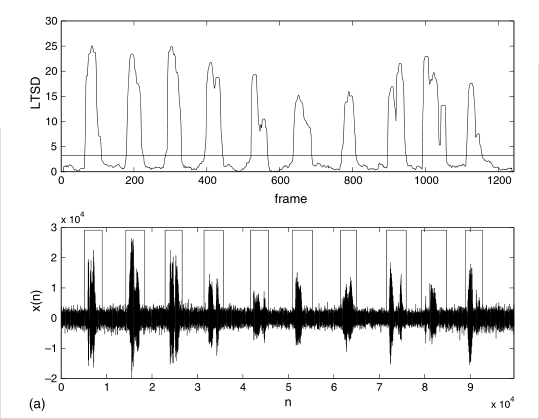
\includegraphics[width=0.6\textwidth]{img/ltsd.png}
        \end{figure}
		Since this is not our primary-task, we shall not expand details here. For further
		information on how these works, please consult original paper.


        %File: feature.tex
%Date: Fri Jan 03 20:48:19 2014 +0800


\subsection{Feature Extraction}

\subsubsection{MFCC}
\label{sec:mfcc}
\textbf{Mel-Frequency Cepstral Coefficient} is a representation of the short-term power spectrum of a sound,
based on a linear cosine transform of a log power spectrum on a nonlinear mel-scale of frequency \cite{mfcc} .
MFCC is the mostly widely used features in Automatic Speech Recognition(ASR), and it can also be applied to Speaker Recognition task.


The process to extract MFCC feature is demonstrated in \figref{mfcc}
\begin{figure}

  \centering
  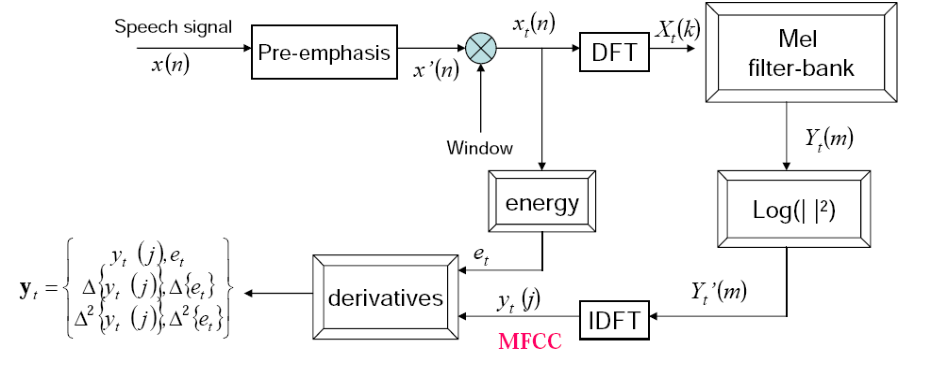
\includegraphics[width=\textwidth]{img/MFCC.png}
  \caption{MFCC feature extraction process\label{fig:mfcc}}

\end{figure}

First, the input speech should be divided into successive short-time frames of length $L$,
neighboring frames shall have overlap $R$.
Those frames are then windowed by Hamming Window, as shown in \figref{framming}.
\begin{figure}
  \centering
  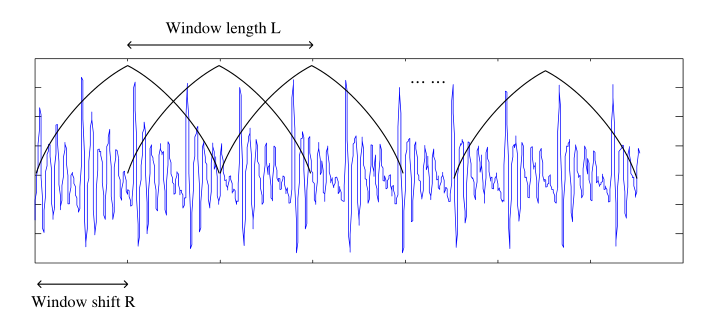
\includegraphics[width=0.7\textwidth]{img/MFCC-windowing-frames.png}
  \caption{Framing and Windowing \label{fig:framming}}
\end{figure}

Then, We perform Discrete Fourier Transform (DFT) on windowed signals to compute their spectrums.
For each of $N$ discrete frequency bands we get a complex number $X[k]$ representing
magnitude and phase of that frequency component in the original signal.

Considering the fact that human hearing is not equally sensitive to all frequency bands, and especially,
it has lower resolution at higher frequencies.
Scaling methods like Mel-scale are aimed at scaling the frequency domain to better fit human auditory perception.
They are approximately linear below 1 kHz and logarithmic above 1 kHz, as shown below in \figref{melscale}:
\begin{figure}[H]
  \centering
  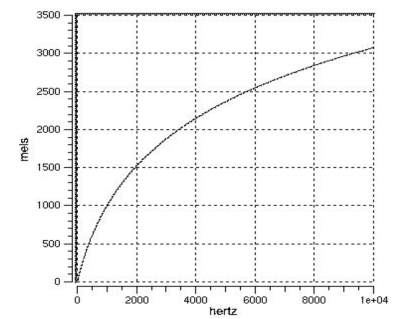
\includegraphics[width=0.5\textwidth]{img/mel-scale.png}
  \caption{Mel-scale plot \label{fig:melscale}}
\end{figure}

In MFCC, Mel-scale is applied on the spectrums of the signals.
The expression of Mel-scale warpping is as followed:
\[ M(f) = 2595 \log_{10}(1 + \dfrac{f}{700}) \]

\begin{figure}[H]
  \centering
  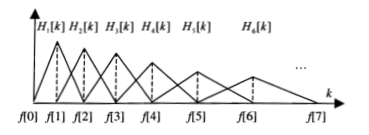
\includegraphics[width=0.5\textwidth]{img/bank.png}
  \caption{Filter Banks (6 filters) \label{fig:bank}}
\end{figure}
Then,  we appply the bank of filters according to Mel-scale on the spectrum,
calculate the logarithm of energy under each bank by $E_i[m] = \log (\sum_{k=0}^{N-1}{X_i[k]^2 H_m[k]}) $ and apply Discrete
Cosine Transform (DCT) on $E_i[m](m = 1, 2, \cdots M) $ to get an array $c_i $:
\[ c_i[n] = \sum_{m=0}^{M-1}{E_i[m]\cos(\dfrac{\pi n}{M}(m - \dfrac{1}{2}))} \]

Then, the first $k$ terms in $c_i $ can be used as features for future training.
The number of $k$ varies in different cases, we will further discuss the choice of $k$ in \secref{result}.

\subsubsection{LPC}
\textbf{Linear predictive coding} is a tool used mostly in audio signal processing and speech
processing for representing the spectral envelope of a
digital signal of speech in compressed form, using the information of a linear predictive model.\cite{lpc}

The basic assumption in LPC is that,
    in a short period, the $n$th signal is a linear combination of previous $p$ signals:
    $ \hat{x}(n) = \sum_{i=1}^pa_i x(n-i)$
    Therefore, to estimate the coefficients $ a_i$, we have to minimize the squared error
    $ \text{E}\left[ \hat{x}(n) - x(n)\right]$.
    This optimization can be done by Levinson-Durbin algorithm.\cite{levinson-durbin}

    Therefore, we first split the input signal into frames, as is done in MFCC feature extraction \secref{mfcc}.
    Then we calculate the $k$ order LPC coefficients for the signal in this frame.
    Since the coefficients is a compressed description for the original audio signal,
    the coefficients is also a good feature for speech/speaker recognition.
    The choice of $k$ will also be further discussed in \secref{result}.


        %File: model.tex
%Date: Fri Jan 03 21:06:49 2014 +0800


\subsection{GMM}
\textbf{Gaussian Mixture Model} is commonly used in acoustic learning task such as speech/speaker recognition,
since it describes the varied distribution of all the feature vector.\cite{GMM}
GMM assumes that the probability of a feature vector $x$ belonging to the model is the following:
\begin{equation}
p(x | w_i, \mu_i, \Sigma_i) = \sum_{i=1}^{K}{w_i \mathcal{N}(x | \mathbf{\mu}_i, \Sigma_i)}
\label{eqn:gmm}
\end{equation}

where
\[\mathcal{N}(x | \mathbf{\mu}_i, \Sigma_i) = \dfrac{1}{(2\pi)^{\frac{d}{2}}\sqrt{|\Sigma_i|}}
\exp \left({-\dfrac{1}{2}(x-\mu_i)^T\Sigma_i^{-1}(x-\mu_i)}\right)\]
subject to
\[\sum_{i=1}^{K} w_i = 1\]

  Therefore, GMM is merely a weighted combination of multivariate Gaussian distribution which
  assumes feature vectors are independent.
  (Actually we use diagonal covariances since the dimensions of the feature vector is independent to each other).
  GMM can describe the distribution of feature vector with several clusters, as shown in \figref{gmm-fig}
\begin{figure}[H]
  \centering
  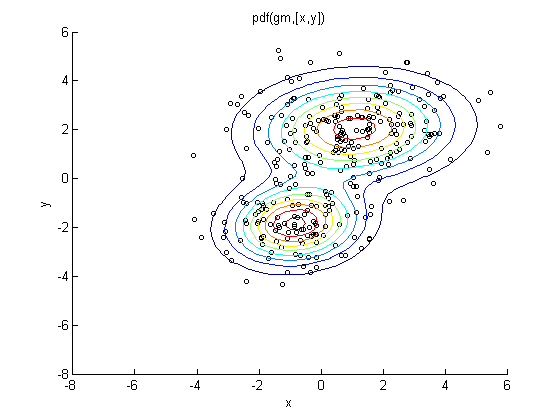
\includegraphics[width=0.8\textwidth]{img/gmm.png}
  \caption{A Two-Dimensional GMM with Two Components\label{fig:gmm-fig}}
\end{figure}

The training of GMM is the process to find the best parameters for $ \mu_i, \Sigma_i, w_i$,
so that the model fits all the training data with maximized likelihood.
More specifically, Expectation-Maximization(EM)
Algorithm\cite{bilmes1998gentle} is used to maximize the likelihood.
The two steps of one iteration of the algorithm in GMM training case here are
\begin{itemize}
	\item \textbf{E-Step} For each data point(feature vector), estimate the probatility that
		each Gaussian generated it\footnote{Actually, for an arbitrary point in
			space, its measure is zero, therefore its ``probability'' is
			actually zero. Therefore, here by ``probability of $x$'' we mean
			``the value of probability distribution function at $x$'' }.
			This is done by direct computation using \eqnref{gmm}.
	\item \textbf{M-Step} Modify the parameters of GMM such that maximize the
		likelihood of data. Here, hidden variable $z_{ij}$ is introduced
		to indicate where $i$-th data point is generate by Gaussian $j$.
		It can be shown that, instead of maximizing the
		likelihood of data, we can maximize the expectation of log likehood
		of data with respect to $Z$.

		let $\theta = \{w, \theta, \Sigma\}$, the log likehood function is
		\[Q(\theta', \theta) = \mathbb{E}_{Z} [\log p(X, Z) | \theta]\]
		where $\theta$ is current parameters, and $\theta'$ is the parameters
		we are to estimate. Incorporating the constraint $\sum_{i=1}^{K} w_i = 1$ using
		Lagrange multiplier gives
		\[J(\theta', \theta) = Q(\theta', \theta) - \lambda\left(\sum_{i=1}^{K} w_i - 1 \right)\]
		Set derivatives to zero, we can get the update equation
		\[Pr(i| x_j) = \dfrac{w_i \mathcal{N}(x_j | \mu_i', \Sigma_i')}{
			\sum_{k=1}^{K} w_k \mathcal{N}(x_j | \mu_k' \Sigma_k')}\]
		\[n_i = \sum_{j=1}^N Pr(i| x_j)\]
		\[\mu_i = \dfrac{1}{n_i} \sum_{t=1}^{T} Pr(i |x_j) x_j\]
		\[\Sigma_i = \left(\dfrac{1}{n_i} \sum_{t=1}^{T} Pr(i |x_j) diag(x_j x_j^T)\right) -
		diag(\mu_i' \mu_i'^T)\]
		\[w_i = \dfrac{n_i}{N}\]

\end{itemize}



After training, the model can give the score of fitness for every input feature vector,
measuring the probability that the vector belongs to this model.

Therefore, in the task of speaker recognition, we can train a GMM for every speaker.
Then for a input signal, we extract lists of feature vectors for it, and calculate the
overall likelihood that the vectors belong to each model.
The speaker whose model fits the input best will be choosen as the answer.

Moreover, an enhancement have been done to the original GMM method.
The training of GMM first requires a random initialization of the means of
all the components. However, we can first use K-Means algorithm\cite{kmeans} to perform a clustering
to all the vectors, then use the clustered centers to initialize the training of GMM.
This enhancement can speed up the training, also gives a better training result.

On the calculation of K-Means, an algorithm call K-MeansII\cite{bahmani2012scalable},
which is an improved version of K-Means++\cite{arthur2007k} can be used for better accuracy.

%\begin{itemize}
  %\item Performance: \\ We investigate the effect of initialization of GMM during
    %training. We implemented GMM with
    %K-meansII\cite{bahmani2012scalable}, which is an improved
    %version of K-means++\cite{arthur2007k} to initialize the
    %mean vector of GMM. Results shows improvements compared
    %to GMM provided by \textbf{scikit-learn\cite{scikit-learn}}.
  %\item Efficiency:
    %\begin{itemize}
      %\item We provide a parallel version of GMM, especially
        %optimized to train large Universal Background Model(UBM).
      %\item We further improve efficiency by utilizing
        %SSE instruction in computing exponential function
        %using polynomial approximation. This can speed up
        %the training procedure by a factor of two.
    %\end{itemize}
%\end{itemize}

\subsection{UBM}

\textbf{Universal Background Model} is a GMM trained on giant number of speakers.
It therefore describes common acoustic features of human voices.\cite{UBM}

As we are providing continuous speech close-set diarization function in
GUI, we adopt \textbf{Universal Background Model} as imposter model using equation
given in \cite{reynolds2000speaker}
and use likelihood ratio test to make reject decisions as proposed in\cite{reynolds2000speaker}.

Further more, by hints mentioned in paper, we only update mean vectors.

When using conversation mode in GUI (will be present later),
GMM model of each user is adapted from a pre-trained UBM
using method described in \cite{reynolds2000speaker}.

\subsection{CRBM}

\textbf{Restricted Boltzmann Machine} is generative stochastic
two-layer neural network that can learn a probability distribution
over its set of binary inputs\cite{rbm_wiki}.  \textbf{Continuous
restricted Boltzmann Machine(CRBM)}\cite{chen2003continuous} extends
its ability to real-valued inputs.  RBM has a ability to, given an
input(visible layer), reconstruct a hidden layer that is similar
to the input.  The neurons
in hidden layer controls the model complexity and the performance of
the network. The Gibbs sampling of hidden layer can be seen as a
representation of the original data. Therefore RBMs can be used
as an auto feature-extractor.
\figref{crbm} illustrate original MFCC data and the
sampled output of reconstructed data from CRBM.

Both RBM and CRBM can be trained using Contrastive Divergence learning,
with subtle difference in update equation.

As details about CRBM are too verbose to be covered here, for interested,
we recommend reading original papers.

Previous works using neural network largely focused on speech
recognition, such as \cite{deep},\cite{mohamed2011deep}.

\begin{figure}[H]
  \begin{minipage}{0.48\linewidth}
    \centering
    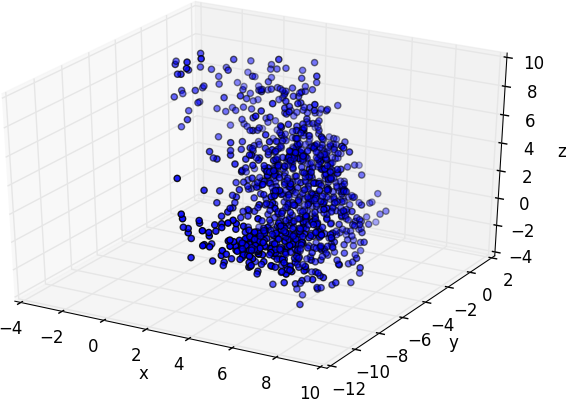
\includegraphics[width=\linewidth]{img/rbm-original.png}
    \caption*{The first three dimension of a woman's MFCC feature}
  \end{minipage}
  \hfill
  \begin{minipage}{0.48\linewidth}
    \centering
    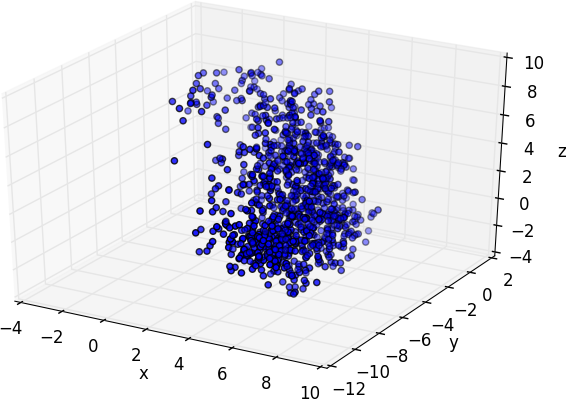
\includegraphics[width=\linewidth]{img/rbm-reconstruct.png}
    \caption*{The first three dimension of the same woman's MFCC feature
      recontructed by a CRBM with 50-neuron hidden layer. We can
      see that, the density of these two distributions are alike}
  \end{minipage}
  \caption{\label{fig:crbm}}
\end{figure}

To use CRBM as a substitution of GMM, rather than
an feature extractor, we train a CRBM per speaker,
and estimate reconstruction error without sampling (which is stable).
The person whose corresponding CRBM has lowest reconstruction error is chosen as

recognition result.

\subsection{JFA}

\textbf{Factor Analysis} is a typical method which behave
very well in classification problems, due to its ability to
account for different types of variability in training data.
Within all the factor analysis methods,
Joint Factor Analysis (JFA)\cite{jfa2,jfa-se} was proved to outperform other method
in the task of Speaker Recognition.

JFA models the user by ``supervector'' , i.e. a $C\times F $ dimension vector, where $C$ is
the number of components in the Universal Background Model, trained by GMM on all the training data,
and $ F$ is the dimension of the acoustic feature vector. The supervector of an utterance is obtained by concatenate
all the $C $ means vectors in the trained GMM model. The basic assumption of JFA on describing a supervector is:

\[ \vec{M} = \vec{ m } + vy + dz + ux, \]

where $m$ is a supervector usually selected to be the one trained from UBM, $v$ is a $ CF \times R_s$ dimension matrix,
$ u$ is a $ CF \times R_c$ dimension matrix, and $d$ is a diagonal matrix.
This four variables are considered independent of all kinds of variabilities and remain constant after training, and
$x, y, z $ are matrixes computed for each utterance sample.
In this formulation, $ m + vy + dz$ is commonly believed to account for the ``Inter-Speaker Variability'', and $ux $ accounts
for the ``Inter-Channel Variability''.
The parameter $ R_s $ and $ R_c$, also referred to as ``Speaker Rank'' and ``Channel Rank'', are two emprical constant selected as first.
The training of JFA is to calculate the best $ u, v, d$ to fit all the training data.




%File: implementation.tex
%Date: Fri Jan 03 21:51:56 2014 +0800


\section{Implementation}
The whole system is written mainly in python, together with some code in C++ and matlab.
The system strongly relies on the support of the numpy\cite{numpy} and scipy\cite{scipy} library.

\begin{enumerate}
    \item VAD

      Three types of  VAD filters are located in \verb|src/filters/|.

      \verb|silence.py| implements an energy-based VAD algorithm.
      \verb|ltsd.py| is a wrapper for LTSD algorithm, relying on pyssp\cite{pyssp}.
      \verb|noisered.py| is a wrapper for SOX noise reduction tools, relying on SOX \cite{sox} being
      installed in the system.

    \item Feature

      Implementations for feature extraction are locaed in \verb|src/feature/|.

      \verb|MFCC.py| is a self-implemented MFCC feature extractor.
      \verb|BOB.py| is a wrapper for the MFCC feature extraction in the bob \cite{bob2012} library.
      \verb|LPC.py| is a LPC feature extractor, relying on \verb|scikits.talkbox| \cite{talkbox}.
      All the three extractor have the same interface, with configurable parameters.

      In the implemention, we have  tried different parameters of these features.
      The test script can be found as \verb|src/test/test-feature.py|
      According to our experiments, we have found that the following parameters are optimal:
      \begin{itemize}
        \item Common parameters:
          \begin{itemize}
            \item Frame size: 32ms
            \item Frame shift: 16ms
            \item Preemphasis coefficient: 0.95
          \end{itemize}
        \item MFCC parameters:
          \begin{itemize}
            \item number of cepstral coefficient: 15
            \item number of filter banks: 55
            \item maximal frequency of the filter bank: 6000
          \end{itemize}
        \item LPC Parameters:
          \begin{itemize}
            \item number of coefficient: 23
          \end{itemize}
      \end{itemize}

    \item GMM

      We have tried GMM from scikit-learn \cite{scikit-learn} as well as pypr \cite{pypr}, but
      they suffer a common problem of inefficency.
      For the consideration of speed, a C++ version of GMM with K-MeansII initialization and
      concurrency support
      was implemented and located in \verb|src/gmm/|. It requires \verb|g++>=4.7| to compile.
      This implementation of GMM also provides a python binding which have similar interface to the GMM in
      scikit-learn.

      The new version of GMM, has enhancement in both speed and accuracy. A more detailed discussion
      will be in \secref{result}.

      At last, we used GMM with 32 components, which is found to be optimal according to our experiment.
      The covariance matrix of every Gaussian component is assumed to be diagonal,
      since each dimension of the feature vector are independent.

    \item CRBM

      CRBM is implemented in C++, located in \verb|src/nn|. It also has concurrency support.

    \item JFA

      From our investigation, we found that the original algorithm \cite{jfa-se} for training JFA model is of
      too much complication and hard to implement.
      Therefore, we use the simpler algorithm presented in \cite{jfa-study}
      to train the JFA model.
      This JFA implementation is based on JFA cookbook\cite{cookbook}.
      To generate feature files for JFA, \verb|test/gen-features-file.py| shall be used.
      After \verb|train.lst, test.lst, enroll.lst| are properly located in \verb|jfa/feature-data|,
      the script \verb|run_all.m| will do the training and testing, and \verb|exp/gen_result.py|
      will calculate the accuracy.

      However, from the result, JFA does not seem to outperform our enhanced MFCC and GMM algorithms
      (but do outperform our old algorithms). It is suspected that the training of a JFA model needs more data than
      we have provided, since JFA needs data from various source to account for different types of variabilities.
      Therefore, we might need to add extra data on the training of JFA, but keep the same data scale in the stage of enrollment,
      to get a better result.

      It is also worth mentioning that the training of JFA will take much longer time than our old method,
      since the estimation process of $ u, v, d$ does not converge quickly. As a result, it might not be practical to add
      JFA approach to our GUI system. But we will still test further on the performance of it, compared to other methods.

    \item GUI

      GUI is implemented based on PyQt\cite{pyqt} and PyAudio\cite{pyaudio}.
      \verb|gui.py| is the entrance point. The usage of GUI will be introduced in \secref{gui}.
  \end{enumerate}


\section{Dataset}
	The dataset provided by teacher comprised of 102 speaker, in which 60 are
	females and the rest are males, with three different speaking style: Spontaneous,
	Reading and Whisper. A statistic is as follows:
	\begin{table}[!ht]
		\centering
		\begin{tabular}{|c|c|c|c|}
			\hline
			& Spontaneous & Reading & Whisper \\\hline
			Average Duration & 202s & 205s & 221s \\\hline
			Female Average Duration & 205s & 202s & 217s \\\hline
			Male Average Duration & 200s & 203s & 223s \\\hline
		\end{tabular}
	\end{table}

\section{Result}
\label{sec:result}
We have tested our method on a corpus provided by teacher Xu. For detailed
description of the corpus, please see former report.

All the tests are conducted serval times (depending on computation cost,
vary from 5 to 20) with random selected training and testing speakers.
The average over these tests are considered as the final
result.

\subsection{Efficiency Test of our GMM}
We have extensively examined the efficiency of our implementation of GMM
compared to scikit-learn version. Test is conducted using real MFCC data with
13 dimensions. We consider the scenario when training a UBM with 256 mixtures.
We examine the time used for ten iteration.  For comparable results, we diabled
the K-means initialization process of both scikit-learn GMM implementation and
ours.  Time used for ten iterations under different data size and concurrency
is recorded.

\begin{figure}[!ht]
	\begin{minipage}{0.48\linewidth}
		\centering
		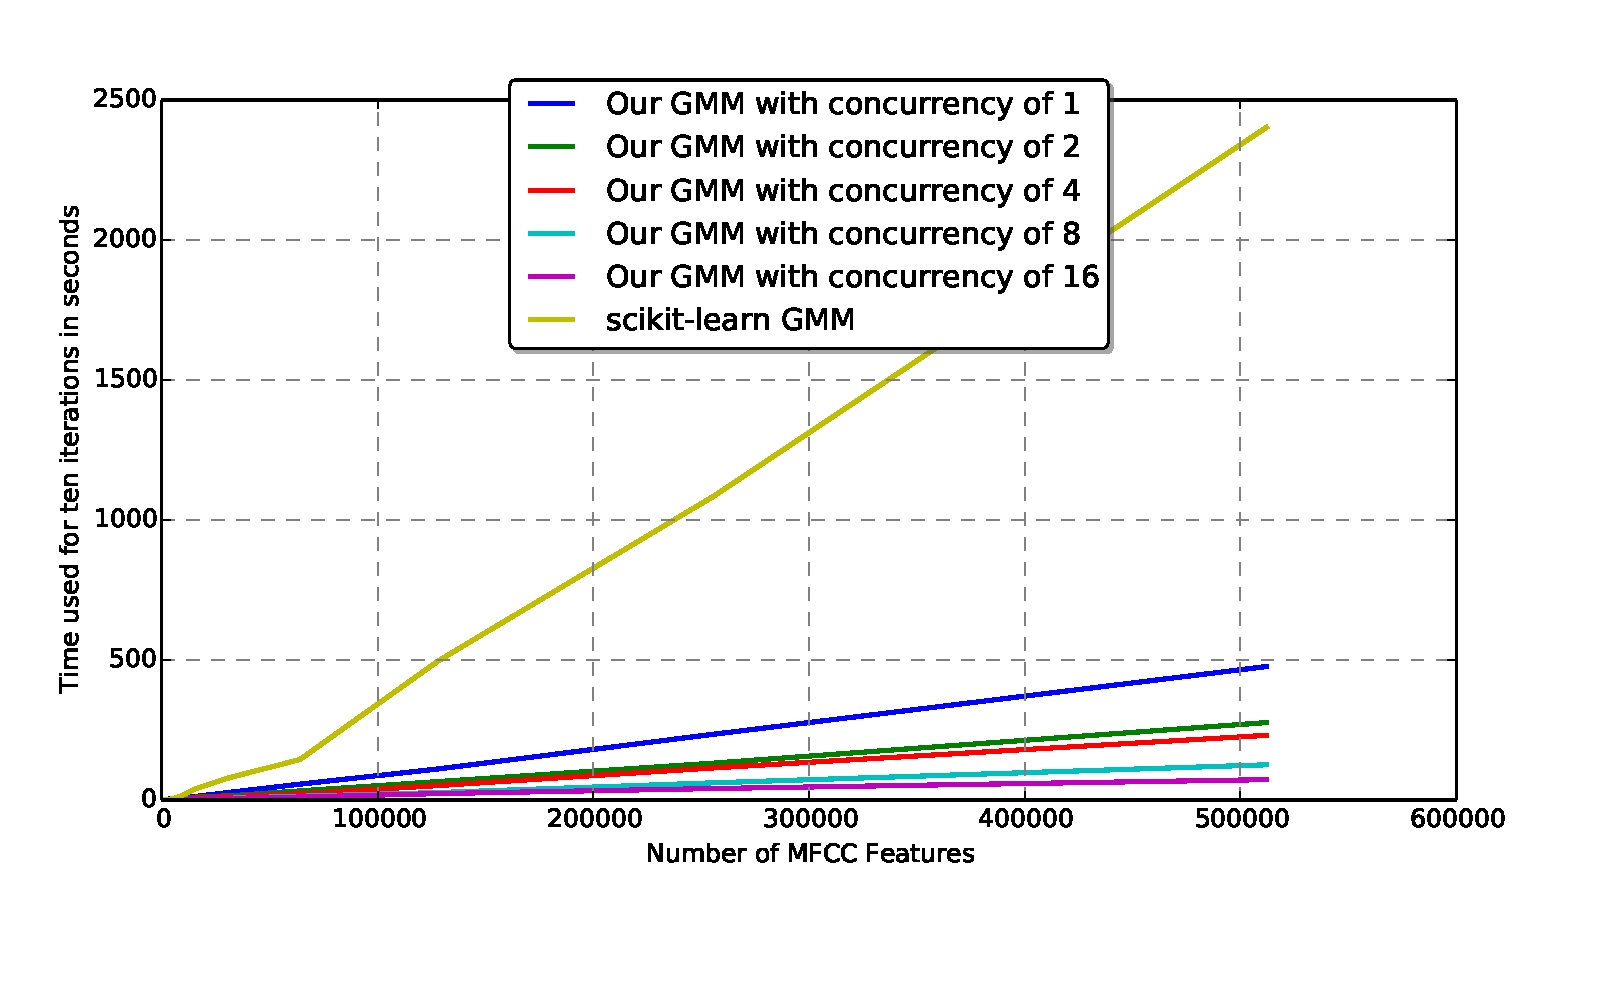
\includegraphics[width=\linewidth]{res/time-comp.pdf}
		\caption{Comparison on efficiency\label{fig:gmm_efficiency}}
	\end{minipage}
	\hfill
	\begin{minipage}{0.48\linewidth}
		\centering
		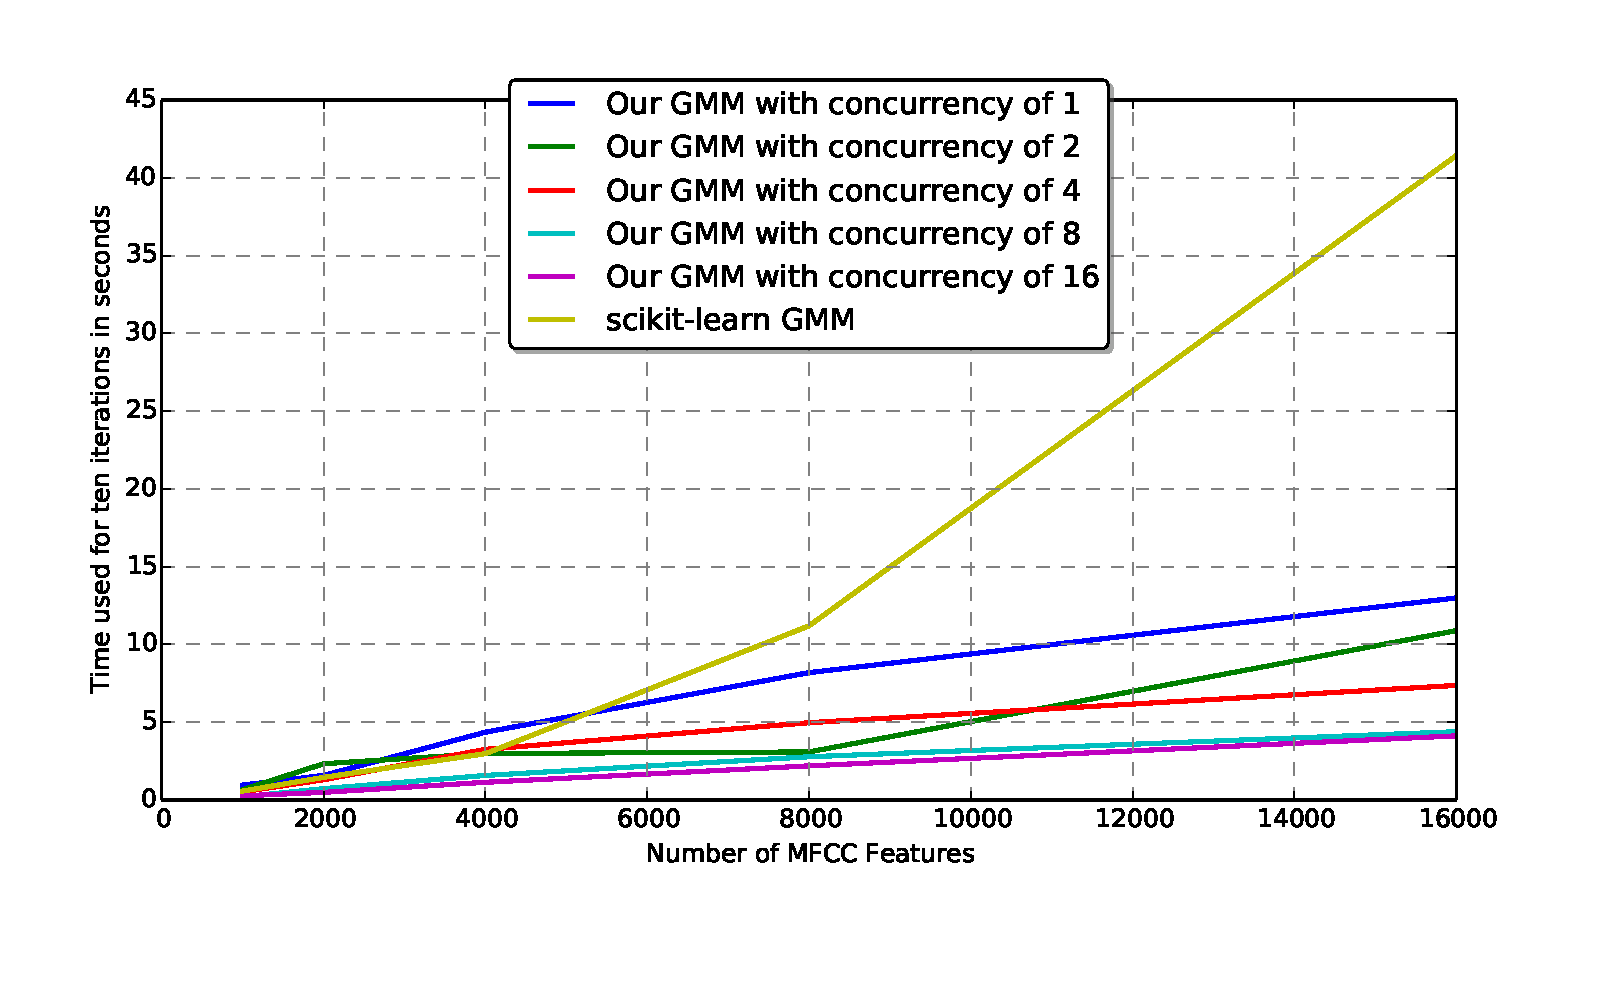
\includegraphics[width=\linewidth]{res/time-comp-small.pdf}
		\caption{Comparison on efficiency when number of MFCC features is small\label{fig:gmm_efficiency_small}}
	\end{minipage}
\end{figure}

From \figref{gmm_efficiency}, we can immediately infer that our method
is much-much more efficient than the widely used version of GMM provided
by scikit-learn when the data size grows sufficiently large.

We shall analyze in two aspect:
\begin{itemize}
	\item No concurrency
		\begin{itemize}
			\item When the number of MFCC features is below 6000, which is a typical
				number of features generated by 60 seconds utterances (1ms frame shift),
				our method is slightly slower; but this is trivial since
				1 minute utterance is too small.
			\item When the number of MFCC features grows sufficiently large, our method
				shows great improvement. When training 512,000 features, our method
				is 5 times faster than comparing method.
		\end{itemize}
	\item With concurrency \\
		Our method shows considerable concurrency scalability that the running time
		is approximately lineary to the number of cores using.

		When using 8-cores, our method is \textbf{$19$ times} faster than comparing
		method.
\end{itemize}


\subsection{Effect Of Number Of Mixtures}
We examined our GMM compared to GMM from scikit-learn.
Test is conducted on 30-speaker corpus, 30 seconds training utterance
and 100 random sampled 5 seconds test utterance for each speaker.

As \figref{mixture} illustrates, when number of mixtures is small,
our GMM outperforms scikit-learn version by $10\%$, which indicates our
GMM models the distribution more accurately. The maximum accuracy
happens when the number of mixtures is around 32, reaching $0.965$. As
the number of mixtures increases, the decrease in accuracy

\begin{figure}
	\centering
	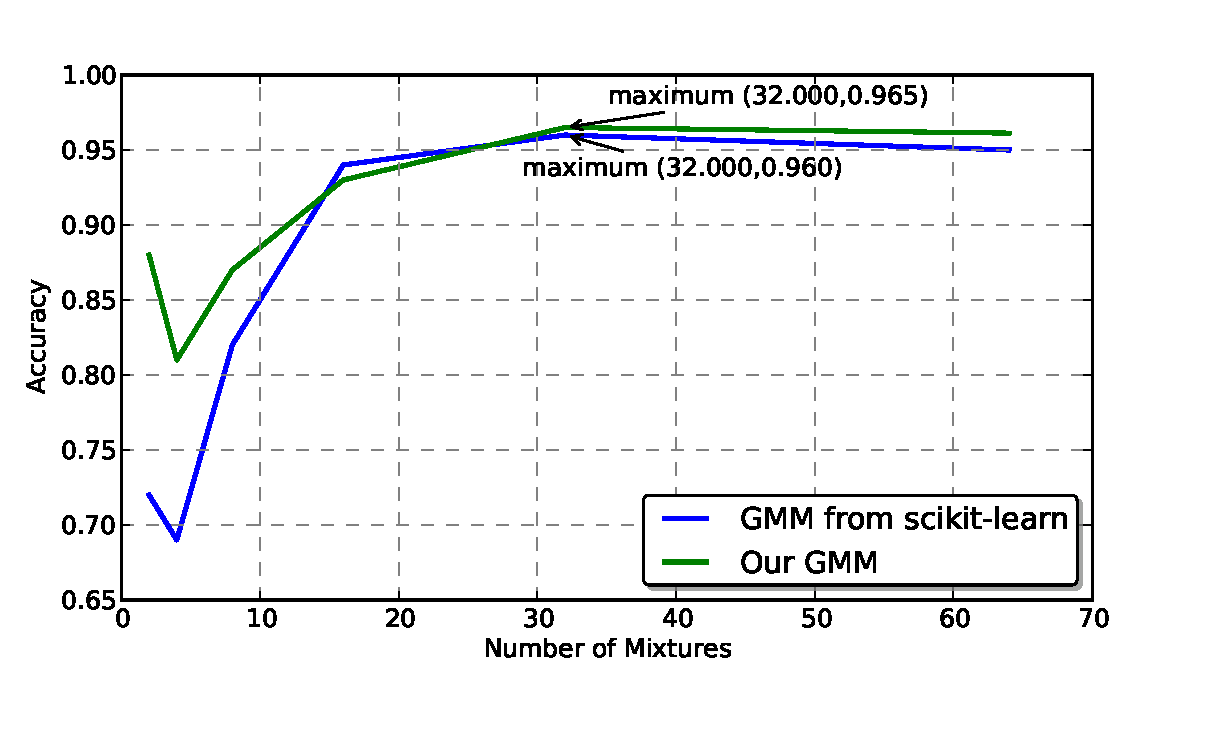
\includegraphics[width=\linewidth]{res/mixture-both.pdf}
	\caption{Accuracy curve on different number of mixtures\label{fig:mixture}}
\end{figure}

\section{Effect On Number Of Speakers}
An apparent trade-off in speaker recognition task is the number of speakers
enrolled and the accuracy of recognizing a person. We've conducted experiments
examining the effect of number of speakers enrolled on the performance of the
system.

The configurations of the test is as followed:
\begin{itemize}
	\item Number of mixtures is set to 32, the optimal number we found previously
	\item GMM from scikit-learn, compared to our GMM.
	\item 30s training utterance and 5s test utterance
	\item 100 sampled test utterance for each user
\end{itemize}


\begin{figure}[!ht]
	\centering
	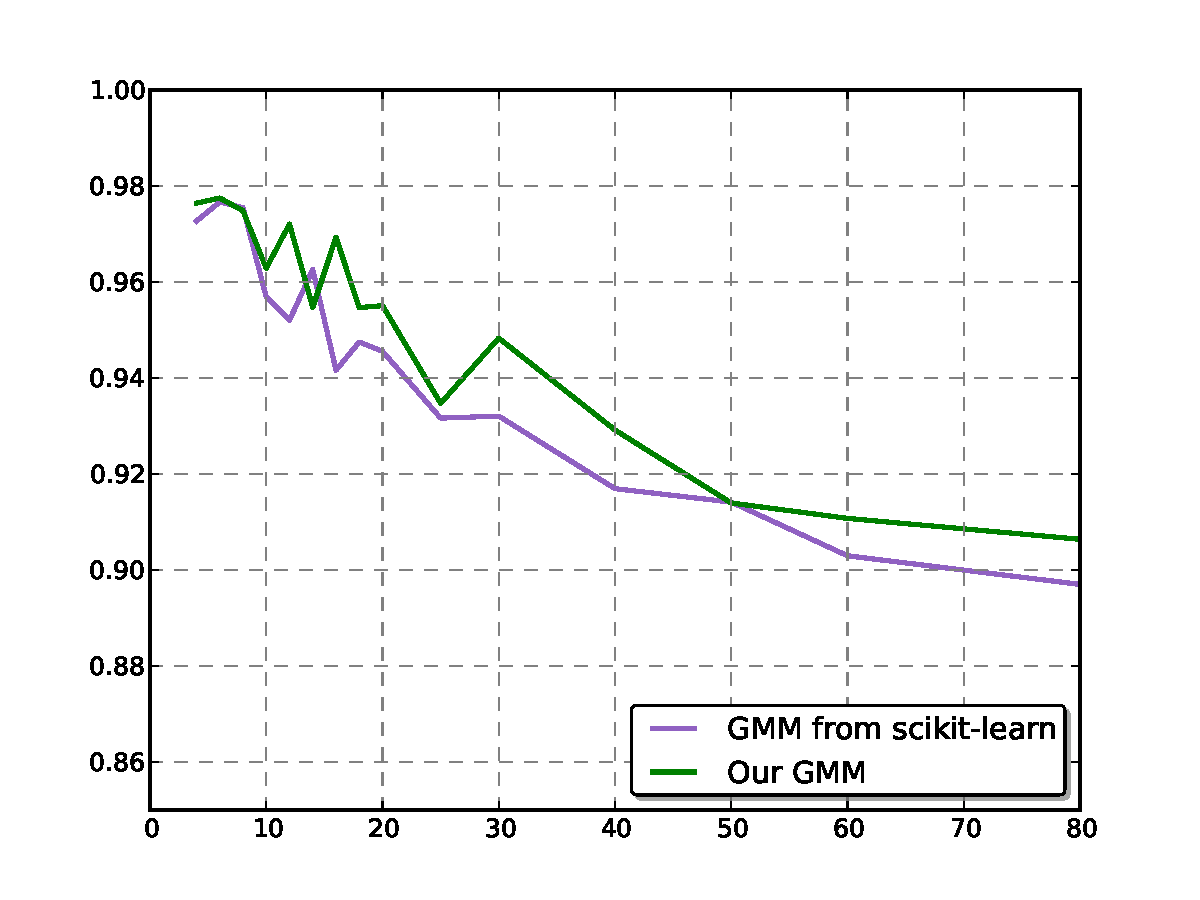
\includegraphics[width=\linewidth]{res/nperson.pdf}
	\caption{Accuracy curve on different number of speakers enrolled\label{fig:nspk_enrolled}}
\end{figure}

Scrunitizing \figref{nspk_enrolled} we would see that, our GMM performs better than
scikit GMM in general. When number of speakers is small, due to the the random
selection, the variance of the tests is significantly high, as we can see from the curve fluctuants.
When number of speakers increases, it is clear that the
accuracy of our GMM is above scikit version. As the more speaker, the more
difficult the recognition task will be, this result suggests that our
optimization on GMM takes effect.



\section{GUI}
	This section describes the design of Graphic User Interface to accomodate our system.
\subsection{Functional Requirements}
	The GUI consists of following functions:
	\begin{itemize}
		\item \textbf{Enrollment of speaker} \\
			A new user can be dynamically add to this system.\
			when enrollment starts, the user is prompted to input
			his identifications, e.g, name, age, sex, a photo would
			be better, and so on.

			Then he is required to record a piece of utterance.
			An article will be prompted to the user in case he/she
			is introrse to say something, he/she can read the article.

			There are two ways to enroll a user:
			\begin{itemize}
				\item \textbf{Enroll by speaking}
					A progress indicator of enrollment process will be present to user.
					When enough utterance is collected, the user will be given
					message about the success of enrollment.

				\item \textbf{Enroll by pre-recorded voice}
					User can upload a pre-recorded voice of a speaker. The system
					accepts the voice given and the enrollment of a speaker is done.
			\end{itemize}

		\item \textbf{Recognition of a user} \\
			A enrolled user present and record a piece of utterance,
			the system tells who the person is.

		\item \textbf{Conversation Recognition mode} \\
			When the system turn into Conversation Recognition mode,
			it will continuously collect voice data, and determine
			who is speaking right now. If a photo is given in previous
			enrollment process, current speaker's photo will show up
			in screen; otherwise the name will be shown.

		\item \textbf{Verification mode} \\
			A user first claim its identity, then the system required
			the user to record a piece of utterance. The system will
			then display whether the speaker is the speaker that claimed
			or an impostor.

			The availability of this function is still under our investigation.

	\end{itemize}

\subsection{Non-Functional Requirements}
	\begin{itemize}
		\item \textbf{Enrollment Efficiency} \\
			The enrollment procedure involves training GMM or RBM model, which
			is a time consuming process. A continuous flow of user enrollment
			should not be interupted.
		\item \textbf{Platform-Independency} \\
			As we program using Python, our program should run on
			platform that supports Python.
		\item \textbf{Recognition Accuracy} \\
			The performance of the system should be good enough to
			make this system could be carried out in practical use.
	\end{itemize}


\printbibliography

\end{document}

